% This file was created with tikzplotlib v0.10.1.
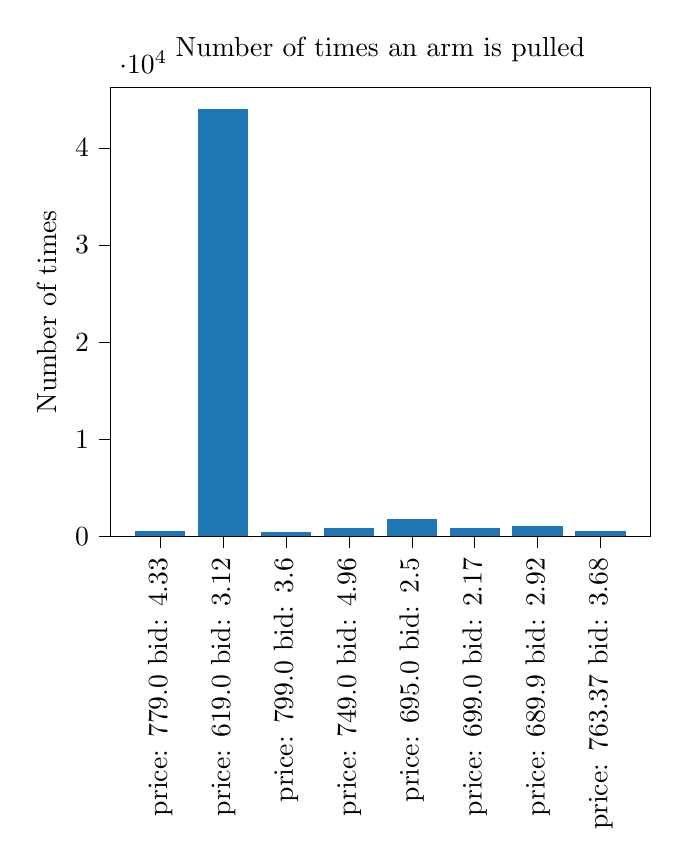
\begin{tikzpicture}

\definecolor{darkgray176}{RGB}{176,176,176}
\definecolor{lightgray204}{RGB}{204,204,204}
\definecolor{steelblue31119180}{RGB}{31,119,180}

\begin{axis}[
legend cell align={left},
legend style={fill opacity=0.8, draw opacity=1, text opacity=1, draw=lightgray204},
tick align=outside,
tick pos=left,
title={Number of times an arm is pulled},
x grid style={darkgray176},
xmin=-0.79, xmax=7.79,
xtick style={color=black},
xtick={0,1,2,3,4,5,6,7},
xticklabel style={rotate=90.0},
xticklabels={
  price: 779.0
bid: 4.33,
  price: 619.0
bid: 3.12,
  price: 799.0
bid: 3.6,
  price: 749.0
bid: 4.96,
  price: 695.0
bid: 2.5,
  price: 699.0
bid: 2.17,
  price: 689.9
bid: 2.92,
  price: 763.37
bid: 3.68
},
y grid style={darkgray176},
ylabel={Number of times},
ymin=0, ymax=46196.85,
ytick style={color=black}
]
\draw[draw=none,fill=steelblue31119180] (axis cs:-0.4,0) rectangle (axis cs:0.4,523);
\draw[draw=none,fill=steelblue31119180] (axis cs:0.6,0) rectangle (axis cs:1.4,43997);
\draw[draw=none,fill=steelblue31119180] (axis cs:1.6,0) rectangle (axis cs:2.4,473);
\draw[draw=none,fill=steelblue31119180] (axis cs:2.6,0) rectangle (axis cs:3.4,850);
\draw[draw=none,fill=steelblue31119180] (axis cs:3.6,0) rectangle (axis cs:4.4,1754);
\draw[draw=none,fill=steelblue31119180] (axis cs:4.6,0) rectangle (axis cs:5.4,820);
\draw[draw=none,fill=steelblue31119180] (axis cs:5.6,0) rectangle (axis cs:6.4,1027);
\draw[draw=none,fill=steelblue31119180] (axis cs:6.6,0) rectangle (axis cs:7.4,556);
\end{axis}

\end{tikzpicture}
